% ------------------------------------------------------------------------------
% It describes the means used to manage a project.
% ------------------------------------------------------------------------------

\opt{never}{\addbibresource{03-tail/bibliography.bib}} % to make citation found in most IDE

\chapter{Project methodology}
\label{chap:methodology}

% -- Your text goes here --
Project methodology consists of describing the means used to manage a project. In this chapter, the concept of agility is described in order to explain how the iterative process works. In addition, the \gls{kanban} methodology is described in detail to explain the time aspect of the tasks to be carried out. Finally, the various tools used are discussed.

\minitoc
\newpage

% ------------------------------------------------------------------------------
\section{Agile methodology}

% -- Your text goes here --
Agile methodology is the main project management method used in this work. It enables the project to be managed from the specifications to the final product. The idea for this method was conceived in the 70s or even before \cite{abbas_historical_2008}.  The idea was to change the development process in software engineering by using iterative techniques. Traditional methods worked with sequential techniques, often called Waterfall. Figure \ref{fig:waterfall_vs_scrum} shows the difference between these two approaches.
\begin{center}
    \begingroup
    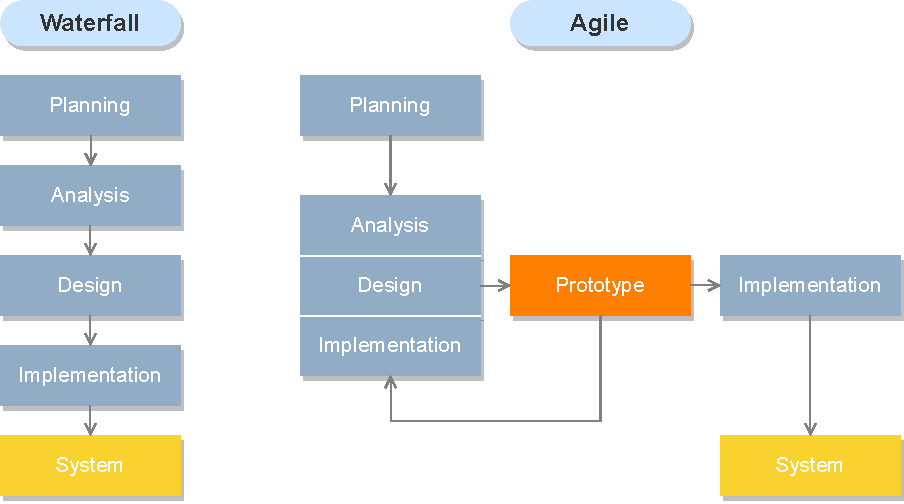
\includegraphics[width=1\columnwidth]{methodology/waterfall_vs_scrum.pdf}
    \captionof{figure}{Sequential and iterative process \cite{course_MA_ITProMan}}
    \label{fig:waterfall_vs_scrum}
    \endgroup
\end{center}
The Waterfall methodology is considered cumbersome. There are deliverables after each phase. Approval is required before moving on to the next phase. It is difficult to go backwards (by moving up the phases). Professors explained this very well during a Masters course given at the \gls{hes} \cite{course_MA_ITProMan}. They added that this method is best used in very large projects where it is difficult to split teams into small groups to work iteratively.

These same teachers \cite{course_MA_ITProMan} described the agile methodology as follows:
\begin{quote}
    \textit{"AGILE" is about values and principles, not practices, but many practices support them. It's not about doing agile, it's about being agile}.
\end{quote}
Several agile process frameworks were created before the 2000s. Examples include \gls{scrum}, XP, RUP, etc. Between the 11th and the 13th of February 2001, 17 people from these different frameworks met to find an alternative to cumbersome, documentation-driven software development processes. They created the agile software development manifesto \cite{manifesto_agile} :
\begin{itemize}
    \item[] \textit{Individuals and interactions over processes and tools}
    \item[] \textit{Working software over comprehensive documentation}
    \item[] \textit{Customer collaboration over contract negotiation}
    \item[] \textit{Responding to change over following a plan}
\end{itemize}
The central principle of agile is to have very rapid iterations to build the first business values. The customer is at the centre of the process thanks to frequent communication with the development team \cite{course_MA_ITProMan}. The process framework chosen for this project is \gls{scrum}. It is very well suited to small projects with small teams. It enables the first software prototypes to be delivered quickly. It adapts easily to changes, unlike a sequential method. It is also based on experience. The idea is to learn continuously through iterations. This is an important point in terms of learning from new developments in the project. This is one of the most popular agile methods. This approach was launched in 1995 by Ken Schwaber and Jeff Sutherland \cite{scrum_guide_site}.

\subsection{\Gls{scrum} roles}
Figure \ref{fig:scrum_roles} shows the different roles in a \gls{scrum} team.
\begin{center}
    \begingroup
    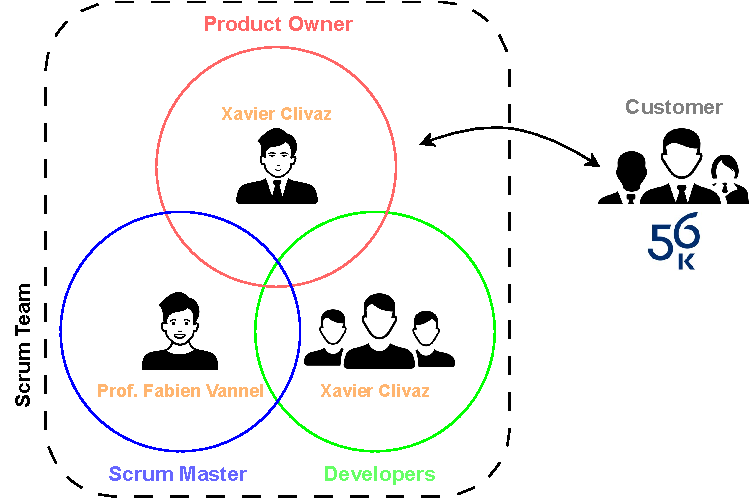
\includegraphics[width=.8\columnwidth]{methodology/scrum_roles.pdf}
    \captionof{figure}{\Gls{scrum} roles}
    \label{fig:scrum_roles}
    \endgroup
\end{center}
A \gls{scrum} guide has been written by Jeff Sutherland and Ken Schwaber to explain the rules \cite{scrum_guide}. First of all, there is the \acrfull{po}. This is the customer's spokesperson. It is he who defines the product's functionalities. They are recorded in a Product Backlog in the form of tasks. He must manage these tasks by prioritising some of them. He is also responsible for the value and return on investment (\acrshort{roi}) of the product. The development team is generally a small one (around seven people \cite{course_MA_ITProMan}). It is capable of self-management. There are no specific roles or positions. Developers have to deal with tasks that are chosen from the Sprint Backlog. Finally, the \gls{scrum} Master is required to be of service to the team. He accompanies the team of developers and prevents obstacles from getting in the way of progress. It is the \gls{scrum} Master who establishes the practices and rules of \gls{scrum}.

\subsection{\texorpdfstring{\gls{scrum}}{} process}
The \gls{scrum} process is relatively simple. It follows the theory described in the official \gls{scrum} guide \cite{scrum_guide}. The life cycle is shown in figure \ref{fig:scrum_process}.
\begin{center}
    \begingroup
    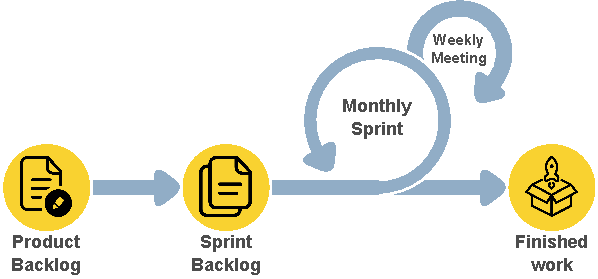
\includegraphics[width=.9\columnwidth]{methodology/scrum_process.pdf}
    \captionof{figure}{\Gls{scrum} life cycle}
    \label{fig:scrum_process}
    \endgroup
\end{center}
The process is made up of multiple elements. It begins on the left of the diagram with the Product Backlog. This is a backlog that is filled by the \acrshort{po}. Since the Product Backlog is generally filled with many functionalities divided into tasks, only one part needs to be selected to be placed in the Sprint Backlog. A Sprint generally corresponds to a period of one month during which the tasks in the Sprint Backlog must be completed. During a Sprint, team meetings are organised every day. These are called Daily Meetings and usually last 15 minutes. A Daily Meeting ensures that, at least once a day, the entire team is available to get support on any problems encountered. In this project, only weekly meetings are held, depending on the distance separating the \gls{scrum} Master and the team of developers. Before each Sprint, a Sprint Planning is carried out to determine the tasks from the Product Backlog to be put into the Sprint Backlog. At the end of a Sprint, an inspection is made of how the Sprint went, with the aim of improving quality and efficiency. This is called a Sprint Retrospective. Finally, it's important to remember that at the end of each Sprint, one stage of the final product is completed. Sometimes this is called an increment.

% ------------------------------------------------------------------------------
\section{KanBan methodology}

% -- Your text goes here --
The \gls{kanban} methodology is very well integrated into \gls{scrum}. Its aim is to manage the workflow as efficiently as possible. According to the \gls{kanban} guide produced by \gls{scrum}.org \cite{kanban_guide}, several fundamental metrics should be taken into account for the flow:
\begin{itemize}
    \item[—] \textbf{\acrfull{wip}} : the number of tasks/items started and not completed.
    \item[—] \textbf{Cycle Time} : the time elapsed between the start and end of a task.
    \item[—] \textbf{Work Item Age} : the time elapsed between the start of the task and now.
    \item[—] \textbf{Throughput} : the number of tasks completed per unit of time.
\end{itemize}
The average cycle time can be predicted using Little's Law \cite{little_law}:
\begin{equation}
    average\ cycle\ time = \frac{average\ \acrshort{wip}}{average\ throughput}
\end{equation}
It explains that the more tasks there are in progress, the longer it will take to complete them. A cycle time in \gls{kanban} can be correlated to a Sprint in the \gls{scrum} methodology. Using this methodology, it is therefore possible to define the right number of tasks for each Sprint Planning. Note that the more you divide a feature into smaller tasks, the easier it will be to predict the cycle time.

\gls{kanban} does more than just limit the \acrshort{wip}. It provides a transparent display of the workflow. Tasks can be represented in a table, as shown in figure \ref{fig:kanban_example}. In this case, the table is virtual and can be viewed from anywhere by the whole \gls{scrum} team.
\begin{center}
    \begingroup
    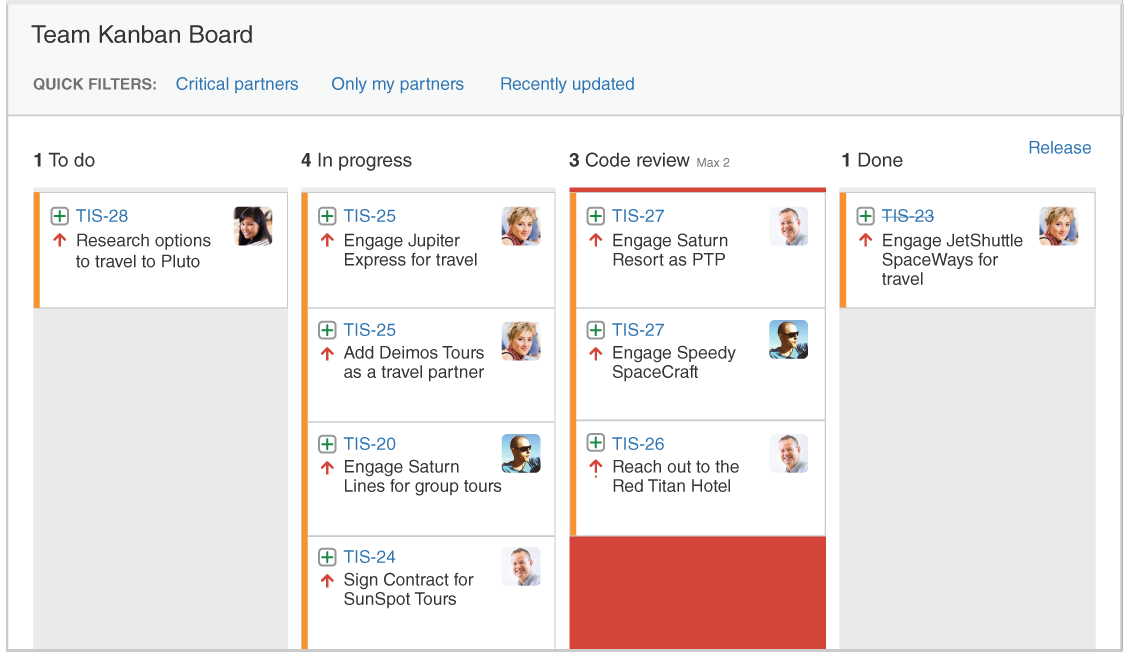
\includegraphics[width=1\columnwidth]{methodology/kanban_example.png}
    \captionof{figure}{Example of a virtual \gls{kanban} table \cite{kanban_example}}
    \label{fig:kanban_example}
    \endgroup
\end{center}
Each label in the table corresponds to a task. A task can contain a priority level and is often assigned to a member of the \gls{scrum} team. All this is defined during Sprint Planning. The labels are categorised in columns to show their progress.


% ------------------------------------------------------------------------------
\section{Project management tools}

% -- Your text goes here --
\subsection{Version control}

\subsection{\acrfull{ci} and \acrfull{cd}}

\subsection{Work packages}


% ------------------------------------------------------------------------------
\section{Formations}

% -- Your text goes here --
\begin{itemize}
    \item AWS Certified Cloud Practitioner
\end{itemize}